

\documentclass[UTF8]{ctexart}
\usepackage{lmodern}
\usepackage{amsmath}
\usepackage{amssymb}
\usepackage{graphicx}
\usepackage{geometry}
\usepackage{color}
\geometry{left=2.18cm,right=2.18cm,top=1.54cm,bottom=2.0cm}
\pagestyle{empty}
\title{\bf 2025春计算方法--实验报告 \#1}
\author{姓名:\underline{~~~~~~~~~~~~~~~~~~~~~~~}  学号:\underline{~~~~~~~~~~~~~~~~~~~~~~~} }
\date{\today}

\begin{document}

\maketitle

运行环境:[自己给出。。。]
%win11,vscode,py3

\section*{实验内容与要求}
\begin{itemize}
  \item{问题1:}
  给定两个函数~$\color{blue}f(x)=\sqrt{x^2+49}-7$~和~$\color{blue}g(x)=\frac{x^2}{\sqrt{x^2+49}+7},$
{\bf\color{red} 采用单精度}(即float型)进行编程~(注意:开方sqrt(x)等内置函数的输出结果默认是双精度,
需要强制转成单精度), 分别取
~$\color{blue}x=4^{-1}, 4^{-2}, 4^{-3}, \cdots, 4^{-11}$,
输出相应的函数值~$\color{blue}f(x)$~和~$\color{blue}g(x)$,
计算结果{\bf 保留12位尾数}(用科学计数形式, 参见表1中的数据格式),比较并分析两种方法得到的计算结果。
你认为哪种方法得到的计算结果更可靠?请给出你的理由或分析。

  \item{问题2:} 给定如下数据


4042.045051380452, 0.000531415926535, -2759471.276702747, 0.0000557052996742895, \\
2755463.874010974, -34.64291531256604,  -0.000031415926535.

分别采取以下4种方式求和:

(a) 顺序求和; ~~~~(b) 逆序(从后往前)求和;

(c) 按绝对值从大到小的顺序, 依次求和;

(d) 按绝对值从小到大的顺序, 依次求和.

采\textbf{\color{red}   用双精度}进行计算,计算结果中的尾数至少保留9位小数(用科学计数形式,比如1.234567899E$-11$).
比较4种方法得到的计算结果;你认为哪种方法得到的计算结果更精确(即误差最小;提示:想办法算出精确值)?
试给出你的理由或分析。


\item{问题3:~(计算结果保留10位有效数字)}  Let $\pi \approx 3.14159 26535 897932.$
\vspace{-0.1in}
\begin{figure}[htb]% 插入两张图片并且并排
	\centering
        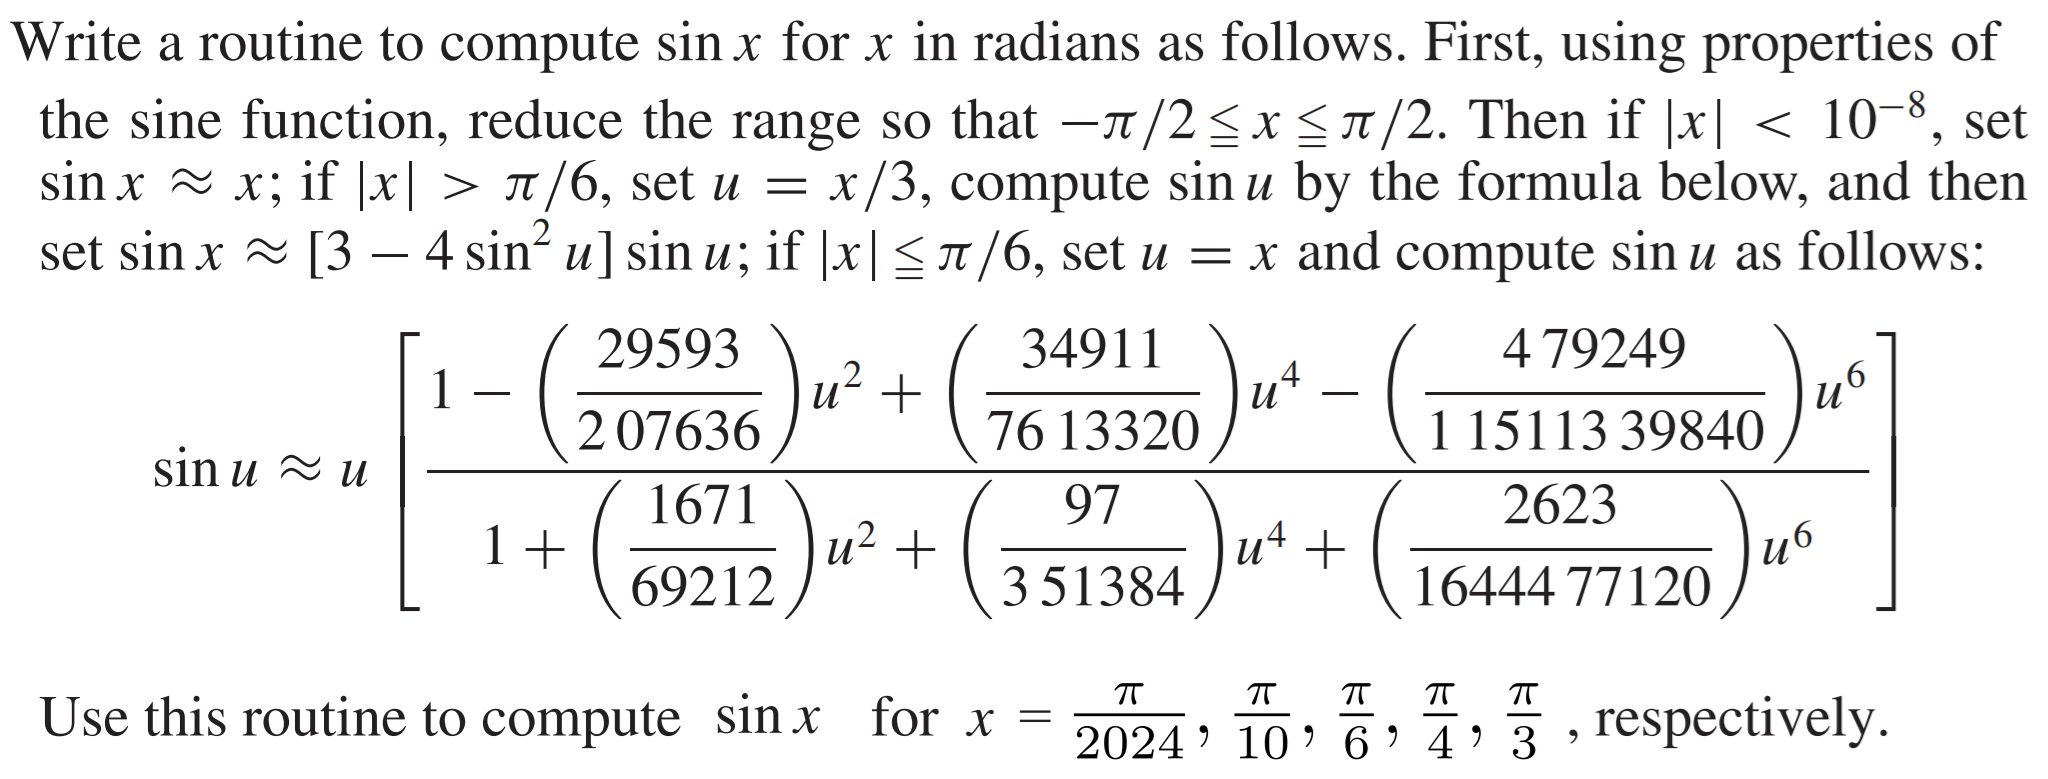
\includegraphics[width=5.40in,height=2.2in, angle=0]{image/lab01c}
  %\caption{\fontsize{9pt}{0pt} N=4 (Left), N=8 (Right)}
\end{figure}

\vspace{-0.2in}
Compare those results with results obtained by the Taylor formula, i.e., $\sin(x) \approx x- \frac{x^3}{3!} +  \frac{x^5}{5!} - \frac{x^7}{7!}$.
\end{itemize}

\clearpage

\section{数值结果(请尽量列表或作图)}
\begin{itemize}
  \item 问题1
\begin{table}[htb]
\begin{center}
\begin{tabular}{|c|c|c|} % 3列,每列居中对齐
\hline
$x$ & $\sqrt{x^2+49}-7$ & $ x^2/(\sqrt{x^2+49}+7)$ \\
\hline
$4^{-1}$=\color{blue}0.250000000000E-000 &\color{blue} 0.\#\#\#\#\#\#\#\#\#\#\#\#E-002 &\color{blue} 0.\#\#\#\#\#\#\#\#\#\#\#\#E-002 \\
\hline
$4^{-2}$=6.250000000000E-002  &  &  \\
\hline
$4^{-3}$ &  &  \\
\hline
$4^{-4}$  &  &  \\
\hline
 &  &  \\
\hline
 &  &  \\
\hline
 &  &  \\
\hline
 &  &  \\
\hline
 &  &  \\
\hline
 &  &  \\
\hline
 &  &  \\
\hline
\end{tabular}
\end{center}
\caption{题1计算结果}
\end{table}


 \item  问题2~(用科学计数形式, 尾数至少保留9位小数)

 \begin{table}[htb]
 \begin{center}
\begin{tabular}{|c|c|c|c|c|c|} % 4列,每列居中对齐
\hline
 & 方法(a) & 方法(b) & 方法(c) & 方法(d) & 精确值 \quad  \\
\hline
Sum & $\quad\quad\quad\quad$ \quad & $\quad\quad\quad\quad\quad $  \quad & \quad$\quad\quad\quad\quad\quad$  & \quad$\quad\quad\quad\quad\quad$  & \\
\hline
\end{tabular}
\end{center}
\caption{题2计算结果}
\end{table}


 \item  问题3~(保留10位有效数字, $\pi \approx 3.14159 26535 897932$)
  \begin{table}[htb]
 \begin{center}
\begin{tabular}{|c|c|c|} % 4列,每列居中对齐
\hline
 $x$  & Special Routine for $\sin(x)$ & Taylor Approximation for $\sin(x)$  \\
\hline
  $\frac{\pi}{2024}$ & $\quad\quad\quad\quad$ \quad & \\
  \hline
  $\frac{\pi}{10}$ & \quad & \\ \hline
  $\frac{\pi}{6}$  & \quad & \\ \hline
  $\frac{\pi}{4}$  &  & \\  \hline
  $\frac{\pi}{3}$  &  & \\
\hline
\end{tabular}
\end{center}
\caption{题3计算结果}
\end{table}

 %$\frac{\pi}{2024}, \frac{\pi}{10}, \frac{\pi}{6}, \frac{\pi}{4}, \frac{\pi}{3}$

\end{itemize}


\section{算法分析}
\vspace{3.50cm}


\section{实验小结}
\vspace{2.0cm}


\end{document}
